\documentclass[11pt]{article}
\usepackage[margin=1in]{geometry}
\usepackage{amsmath,amssymb}
\usepackage{booktabs}
\usepackage{graphicx}
\usepackage{enumitem}

\title{CS555 HW1 -- Question 2: Growth Factors}
\author{}
\date{}

\begin{document}
\maketitle

%----------------------------------------------------------------------
\section*{2a. Asymptotic value of the CN growth factor}
%----------------------------------------------------------------------

Consider the model ODE $\frac{du}{dt} = \lambda u$, with $\lambda \in \mathbb{R}$
and $\lambda < 0$ for stability.

The Crank--Nicolson scheme applied to this ODE gives:
\[
  \frac{u^{n+1} - u^{n}}{\Delta t}
  = \frac{\lambda}{2}\bigl(u^{n+1} + u^{n}\bigr).
\]

Rearranging to solve for $u^{n+1}$:
\[
  u^{n+1} - \frac{\lambda\Delta t}{2}\,u^{n+1}
  = u^{n} + \frac{\lambda\Delta t}{2}\,u^{n},
\]
\[
  u^{n+1}\!\left(1 - \frac{\lambda\Delta t}{2}\right)
  = u^{n}\!\left(1 + \frac{\lambda\Delta t}{2}\right).
\]

Therefore the growth factor is:
\[
  \boxed{G(\lambda\Delta t)
  = \frac{u^{n+1}}{u^{n}}
  = \frac{1 + \lambda\Delta t/2}{1 - \lambda\Delta t/2}.}
\]

Let $z = \lambda\Delta t$. We seek the limit as $z \to -\infty$:
\[
  G(z) = \frac{1 + z/2}{1 - z/2}.
\]

Dividing numerator and denominator by $z/2$:
\[
  G(z) = \frac{\frac{2}{z} + 1}{\frac{2}{z} - 1}.
\]

As $z \to -\infty$, $\frac{2}{z} \to 0$, so:
\[
  \boxed{\lim_{z \to -\infty} G(z)
  = \frac{0 + 1}{0 - 1} = -1.}
\]

\medskip\noindent\textbf{Interpretation:}
As $\lambda\Delta t \to -\infty$ (i.e., very stiff problems or large time steps),
the CN growth factor approaches $-1$.
This means high-frequency modes are \emph{not} damped; instead they oscillate
with alternating sign at each time step with $|G| \approx 1$.
This is why CN is \textbf{A-stable} ($|G| \le 1$ for all $\lambda\Delta t \le 0$)
but \textbf{not L-stable} ($G \not\to 0$ as $\lambda\Delta t \to -\infty$).

In contrast, Euler Backward has $G = 1/(1-z) \to 0$ as $z \to -\infty$,
making it L-stable and better suited for non-smooth initial conditions.

\newpage
%----------------------------------------------------------------------
\section*{2b. Growth factor plot}
%----------------------------------------------------------------------

The growth factors for the four time steppers applied to $du/dt = \lambda u$ are:

\begin{align*}
  \text{Analytical:}        &\quad G = e^{\lambda\Delta t}, \\[4pt]
  \text{Euler Forward (EF):} &\quad G = 1 + \lambda\Delta t, \\[4pt]
  \text{Euler Backward (EB):}&\quad G = \frac{1}{1 - \lambda\Delta t}, \\[4pt]
  \text{Crank--Nicolson (CN):}&\quad G = \frac{1 + \lambda\Delta t/2}{1 - \lambda\Delta t/2}.
\end{align*}

\begin{figure}[h!]
\centering
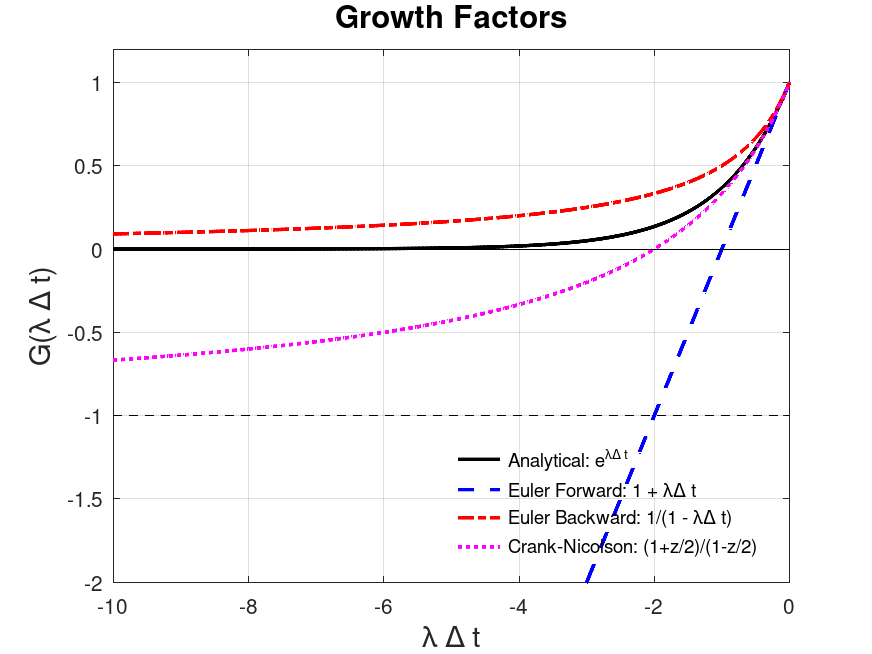
\includegraphics[width=0.85\textwidth]{plot_q2b.png}
\caption{Growth factors $G(\lambda\Delta t)$ for $-10 \le \lambda\Delta t \le 0$.
         The dashed black line marks $G = -1$.}
\end{figure}

\noindent\textbf{Observations:}
\begin{itemize}[nosep]
  \item \textbf{Analytical} ($e^z$): The exact growth factor decays monotonically
        from 1 to 0 as $z \to -\infty$. This is the ideal behavior---all decaying
        modes should be damped.
  \item \textbf{Euler Forward} ($1+z$): Matches the analytical solution near $z=0$
        (1st-order tangent), but becomes \emph{unstable} ($|G|>1$) for $z < -2$.
        This is the well-known CFL stability restriction of explicit methods.
  \item \textbf{Euler Backward} ($1/(1-z)$): Always positive and $|G|<1$ for all
        $z<0$ (A-stable). Moreover, $G \to 0$ as $z \to -\infty$ (\textbf{L-stable}),
        meaning it strongly damps high-frequency/stiff modes. However, it is only
        1st-order accurate.
  \item \textbf{Crank--Nicolson} ($(1+z/2)/(1-z/2)$): A-stable with $|G| \le 1$
        for all $z \le 0$, and 2nd-order accurate. However, $G \to -1$ as
        $z \to -\infty$ (\textbf{not L-stable}). The negative sign means
        high-frequency modes alternate in sign each time step, producing
        oscillations rather than being damped. This explains the oscillatory
        behavior observed with the square-wave IC in Question~1b.
\end{itemize}

\end{document}
